% LaTeX mintafájl szakdolgozat és diplomamunkáknak az
% SZTE Informatikai Tanszékcsoportja által megkövetelt
% formai követelményeinek megvalósításához
% Modosítva: 2011.04.28 Nemeth L. Zoltan
% A fájl használatához szükséges a magyar.ldf 2005/05/12 v1.5-ös vagy későbbi verziója
% ez letölthető a http://www.math.bme.hu/latex/ weblapról, a magyar nyelvű szedéshez
% Hasznos információk, linekek, LaTeX leírások a www.latex.lap.hu weboldalon vannak.
%

\documentclass[12pt]{report}

%Magyar nyelvi támogatás (Babel 3.7 vagy későbbi kell!)
\def\magyarOptions{defaults=hu-min}
\usepackage[magyar]{babel}

%Az ékezetes betűk használatához:
\usepackage{t1enc}% ékezetes szavak automatikus elválasztásához
\usepackage[utf8]{inputenc}% ékezetes szavak beviteléhez

% A formai kovetelmenyekben megkövetelt Times betűtípus használata:
\usepackage{times}

%Az AMS csomagjai
\usepackage{amsmath}
\usepackage{amssymb}
\usepackage{amsthm}

%A fejléc láblécek kialakításához:
\usepackage{fancyhdr}

%Természetesen további csomagok is használhatók,
%például ábrák beillesztéséhez a graphix és a psfrag,
%ha nincs rájuk szükség természetesen kihagyhatók.
\usepackage{graphicx}
\usepackage{psfrag}

\usepackage{setspace}

\usepackage{hyperref}
\hypersetup{
    colorlinks,
    citecolor=black,
    filecolor=black,
    linkcolor=black,
    urlcolor=black
}

\usepackage{cite}

%\usepackage{enumitem}
\usepackage{enumerate}

% Színek
\usepackage{color}
\definecolor{myCommentColorGreen}{RGB}{0,128,0}
\definecolor{myLineNumberGray}{RGB}{128,128,128}

% Forráskódhoz
\usepackage{listings}
\lstset{ %
    %backgroundcolor=\color{white},   % choose the background color; you must add  \usepackage{color} or \usepackage{xcolor}
    basicstyle=\footnotesize,         % the size of the fonts that are used for    the code
    %breakatwhitespace=false,         % sets if automatic breaks should only      happen at whitespace
    breaklines=true,                  % sets automatic line breaking          captionpos=b,                    % sets the caption-position to          bottom
    commentstyle=\color{myCommentColorGreen},    % comment style
    %deletekeywords={...},            % if you want to delete keywords              from the given language
    %escapeinside={\%*}{*)},          % if you want to add LaTeX                within your code
    %extendedchars=true,              % lets you use non-ASCII                  characters; for 8-bits encodings only, does not work with                  UTF-8
    frame=leftline,                   % adds a frame around the                    code
    %keepspaces=true,                 % keeps spaces in text,                      useful for keeping indentation of code (possibly needs                      columns=flexible)
    inputpath=../../../code/gepard,
    keywordstyle=\color{blue},        % keyword style
    language=C++,                     % the language of                          the code
    %morekeywords={*,...},            % if you want to                            add more keywords to the set
    numberfirstline=true,
    numbers=left,                     % where to put                              the line-numbers; possible values are (none, left, right)
    numbersep=10pt,                   % how far theline-numbers are from the code
    numberstyle=\tiny\color{myLineNumberGray}, % the stylethat is used for the line-numbers
    %name=\thelstnumber,              %
    %rulecolor=\color{black},         % if notset, the frame-color may be changed online-breaks within not-black text (e.g.comments (green here))
    %showspaces=false,                % showspaces everywhere adding particularunderscores; it overrides'showstringspaces'
    %showstringspaces=false,          % underline spaces within strings only
    %showtabs=false,                  % show tabs within strings addingparticular underscores
    %stepnumber=2,                    % the step between two line-numbers.If it's 1, each line will benumbered
    %stringstyle=\color{mymauve},     % string literal style
    tabsize=4,                        % sets default tabsize to 2    spaces
    %title=\lstname                   % show the filename of     files included with     \lstinputlisting; also try     caption instead of title
}

% Kép mellett folyó íráshoz
\usepackage{wrapfig}

%Tételszerű környezetek definiálhatók, ezek most fejezetenként együtt számozódnak, pl.
\newtheorem{tét}{Tétel}[chapter]
\newtheorem{defi}[tét]{Definíció}
\newtheorem{lemma}[tét]{Lemma}
\newtheorem{áll}[tét]{Állítás}
\newtheorem{köv}[tét]{Következmény}

%Ha a megjegyzések és a példak szövegét nem akarjuk dőlten szedni, akkor
%az alábbi parancs után kell őket definiální:
\theoremstyle{definition}
\newtheorem{megj}[tét]{Megjegyzés}
\newtheorem{pld}[tét]{Példa}

%%% Saját parancsok
% Az angol kifejezések kiemelése
\newcommand{\inenglish}[1]{\textsl{#1}}
\newcommand{\inenglishfn}[1]{\footnotesize{\inenglish{#1}}}

%\hyphenation{sza-bály el-kü-lö-ní-tett}

%Margók:
\hoffset -1in
\voffset -1in
\oddsidemargin 35mm
\textwidth 150mm
\topmargin 15mm
\headheight 10mm
\headsep 5mm
\textheight 237mm

\begin{document}


%%%%%%%%%%%%%%%%%%%%%%%%%%%%%%%%%%%%%%%%%%%%%%%%%%%%%%%%%%%%%%%%%%%%%%
%%   Címlap                                                         %%
%%%%%%%%%%%%%%%%%%%%%%%%%%%%%%%%%%%%%%%%%%%%%%%%%%%%%%%%%%%%%%%%%%%%%%

    %A FEJEZETEK KEZDŐOLDALAINAK FEJ ÉS LÁBLÉCE:
    %a plain oldalstílust kell átdefiniálni, hogy ott ne legyen fejléc:
    \fancypagestyle{plain}{%
    %ez mindent töröl:
    \fancyhf{}
    % a láblécbe jobboldalra kerüljön az oldalszám:
    \fancyfoot[R]{\thepage}
    %elválasztó vonal sem kell:
    \renewcommand{\headrulewidth}{0pt}
    }

    %A TÖBBI OLDAL FEJ ÉS LÁBLÉCE:
    \pagestyle{fancy}
    \fancyhf{}
    \fancyhead[L]{<Cím>}
    \fancyfoot[R]{\thepage}


    %A címoldalra se fej- se lábléc nem kell:
    \thispagestyle{empty}

    \begin{center}
    \vspace*{1cm}
    {\Large\bf Szegedi Tudományegyetem}

    \vspace{0.5cm}

    {\Large\bf Informatikai Tanszékcsoport}

    \vspace*{3.8cm}

    % Tíz sorral fentebb is át kell írni!!!
    {\LARGE\bf Cím}


    \vspace*{3.6cm}

    {\Large Szakdolgozat}
    % vagy {\Large Diplomamunka}

    \vspace*{4cm}

    %Értelemszerűen megváltoztatandó:
    {\large
    \begin{tabular}{c@{\hspace{4cm}}c}
    \emph{Készítette:}     &\emph{Témavezető:}\\
    \bf{<Hallgató>}  &\bf{<Oktató>}\\
    informatika szakos     & <oktatói beosztás>\\
    hallgató &
    \end{tabular}
    }

    \vspace*{2.3cm}

    {\Large
    Szeged
    \\
    \vspace{2mm}
    <év>
    }
    \end{center}


    % 1.5-ös sorköz:
    % ezt javasolják:  \linespread{1.25}
    % és ez bevált, de ehhez kellett a \usepackage{setspace} csomag betöltése.
    \onehalfspacing


%%%%%%%%%%%%%%%%%%%%%%%%%%%%%%%%%%%%%%%%%%%%%%%%%%%%%%%%%%%%%%%%%%%%%%
%%   Tartalomjegyzék                                                %%
%%%%%%%%%%%%%%%%%%%%%%%%%%%%%%%%%%%%%%%%%%%%%%%%%%%%%%%%%%%%%%%%%%%%%%

    \tableofcontents


%%%%%%%%%%%%%%%%%%%%%%%%%%%%%%%%%%%%%%%%%%%%%%%%%%%%%%%%%%%%%%%%%%%%%%
%%   Feladatkiírás                                                  %%
%%%%%%%%%%%%%%%%%%%%%%%%%%%%%%%%%%%%%%%%%%%%%%%%%%%%%%%%%%%%%%%%%%%%%%


    %A \chapter* parancs nem ad a fejezetnek sorszámot
    \chapter*{Feladatkiírás}
    %A tartalomjegyzékben mégis szerepeltetni kell, mint szakasz(section) szerepeljen:
    \addcontentsline{toc}{section}{Feladatkiírás}

A témavezető által megfogalmazott feladatkiírás. Önálló oldalon szerepel.


%%%%%%%%%%%%%%%%%%%%%%%%%%%%%%%%%%%%%%%%%%%%%%%%%%%%%%%%%%%%%%%%%%%%%%
%%   Tartalmi összefoglaló                                          %%
%%%%%%%%%%%%%%%%%%%%%%%%%%%%%%%%%%%%%%%%%%%%%%%%%%%%%%%%%%%%%%%%%%%%%%

    \chapter*{Tartalmi összefoglaló}
    \addcontentsline{toc}{section}{Tartalmi összefoglaló}

%A tartalmi összefoglalónak tartalmaznia kell (rövid, legfeljebb egy oldalas, összefüggő megfogalmazásban)
%a következőket: a téma megnevezése, a megadott feladat megfogalmazása - a feladatkiíráshoz viszonyítva-,
%a megoldási mód, az alkalmazott eszközök, módszerek, az elért eredmények, kulcsszavak (4-6 darab).

%Az összefoglaló nyelvének meg kell egyeznie a dolgozat nyelvével. Ha a dolgozat idegen nyelven készül,
%magyar nyelvű tartalmi összefoglaló készítése is kötelező (külön lapon), melynek terjedelmét a TVSZ szabályozza.

    \subsubsection*{A téma megnevezése}

    \subsubsection*{A megadott feladat megfogalmazása}

    \subsubsection*{A megoldásmód}

    \subsubsection*{Alkalmazott eszközök, módszerek}

    \subsubsection*{Elért eredmények}

    \subsubsection*{Kulcsszavak}


%%%%%%%%%%%%%%%%%%%%%%%%%%%%%%%%%%%%%%%%%%%%%%%%%%%%%%%%%%%%%%%%%%%%%%
%%   Bevezetés                                                      %%
%%%%%%%%%%%%%%%%%%%%%%%%%%%%%%%%%%%%%%%%%%%%%%%%%%%%%%%%%%%%%%%%%%%%%%

    \chapter*{Bevezetés}
    \label{Bevezetés}
    \addcontentsline{toc}{section}{Bevezetés}


%%%%%%%%%%%%%%%%%%%%%%%%%%%%%%%%%%%%%%%%%%%%%%%%%%%%%%%%%%%%%%%%%%%%%%
%%   Háttér                                                         %%
%%%%%%%%%%%%%%%%%%%%%%%%%%%%%%%%%%%%%%%%%%%%%%%%%%%%%%%%%%%%%%%%%%%%%%

    \chapter{Háttér}
    \label{Háttér}


%%%%%%%%%%%%%%%%%%%%%%%%%%%%%%%%%%%%%%%%%%%%%%%%%%%%%%%%%%%%%%%%%%%%%%
%%   <Téma>                                                         %%
%%%%%%%%%%%%%%%%%%%%%%%%%%%%%%%%%%%%%%%%%%%%%%%%%%%%%%%%%%%%%%%%%%%%%%

    \chapter{<Téma>\cite{Cabanier:14:HCC}}

    \lstinputlisting[language=C++, firstline=40, lastline=65]{src/gepard.h}

    \begin{figure}[h]
    \centering
    \psfrag{t}[c][c]{$q_0$}
    \centerline{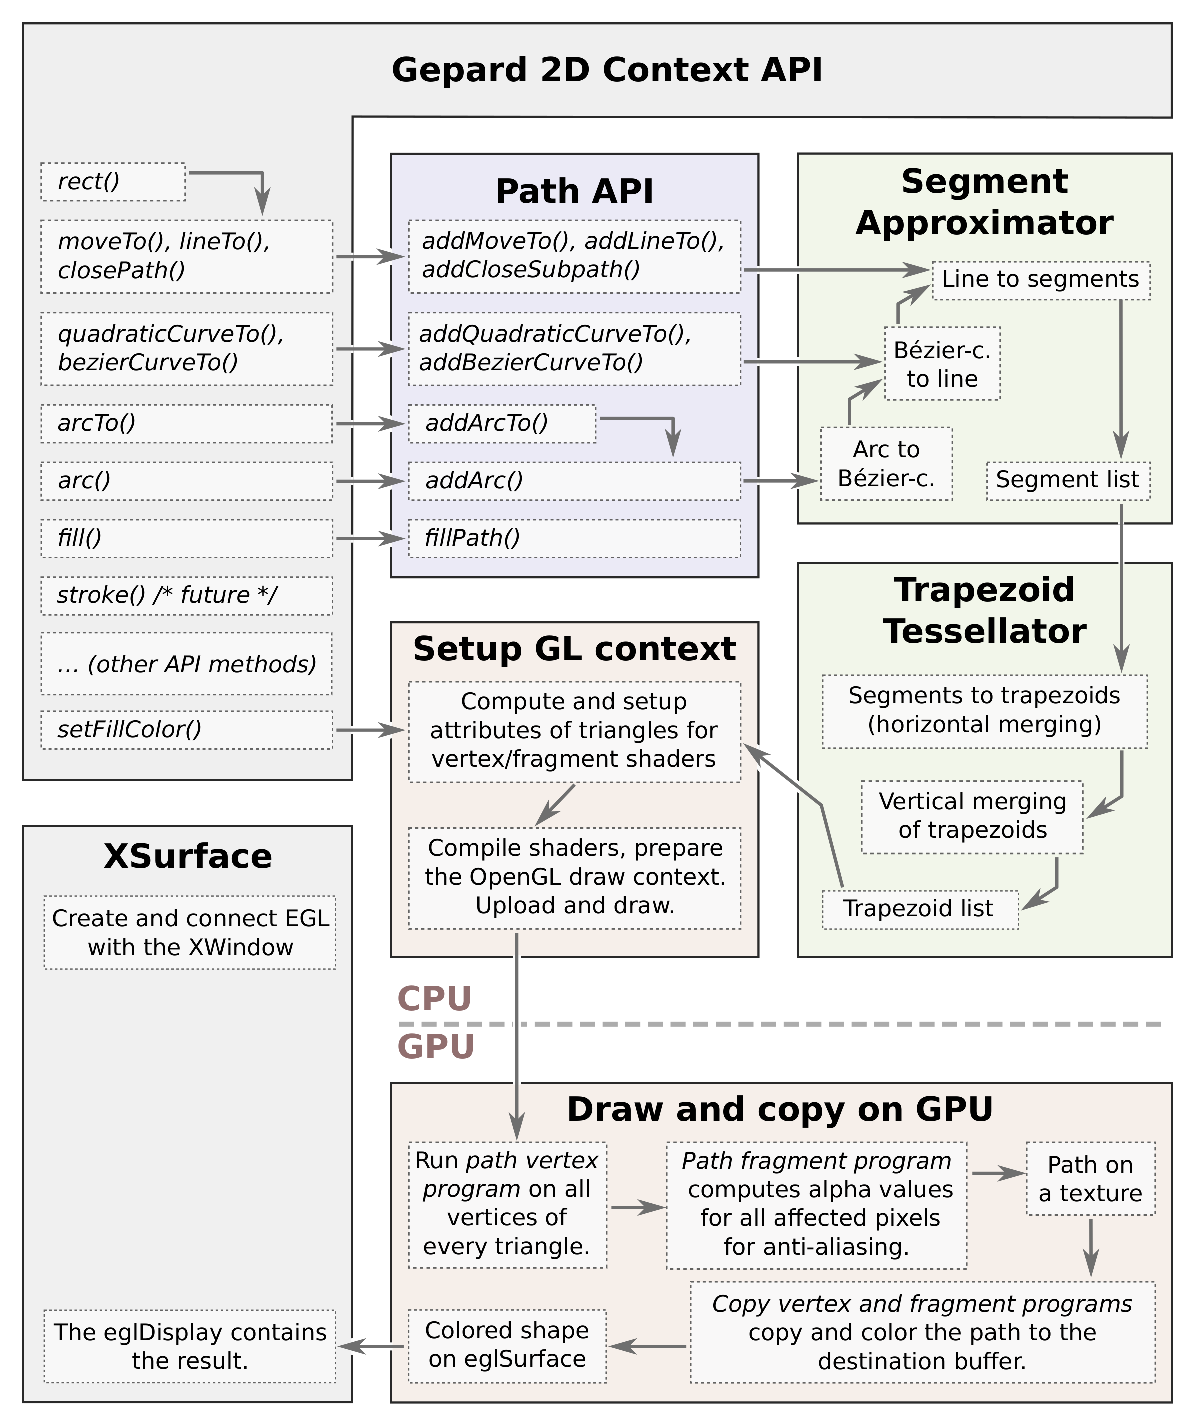
\includegraphics[scale=0.6]{img/dataflow_eps}}
    \caption{\label{dataflow-diagram} A rajzolás folyamata}
    \end{figure}


%%%%%%%%%%%%%%%%%%%%%%%%%%%%%%%%%%%%%%%%%%%%%%%%%%%%%%%%%%%%%%%%%%%%%%
%%   Konklúzió                                                      %%
%%%%%%%%%%%%%%%%%%%%%%%%%%%%%%%%%%%%%%%%%%%%%%%%%%%%%%%%%%%%%%%%%%%%%%

    \chapter{Konklúzió}
    \addcontentsline{toc}{section}{Konklúzió}


%%%%%%%%%%%%%%%%%%%%%%%%%%%%%%%%%%%%%%%%%%%%%%%%%%%%%%%%%%%%%%%%%%%%%%
%%   Irodalomjegyzék                                                %%
%%%%%%%%%%%%%%%%%%%%%%%%%%%%%%%%%%%%%%%%%%%%%%%%%%%%%%%%%%%%%%%%%%%%%%

    \bibliography{bib/cites}{}
    \bibliographystyle{bib/huplain}

%%%%%%%%%%%%%%%%%%%%%%%%%%%%%%%%%%%%%%%%%%%%%%%%%%%%%%%%%%%%%%%%%%%%%%
%%   Nyilatkozat                                                    %%
%%%%%%%%%%%%%%%%%%%%%%%%%%%%%%%%%%%%%%%%%%%%%%%%%%%%%%%%%%%%%%%%%%%%%%

    \chapter*{Nyilatkozat}
    %Egy üres sort adunk a tartalomjegyzékhez:
    \addtocontents{toc}{\ }
    \addcontentsline{toc}{section}{Nyilatkozat}
    %\hspace{\parindent}

    % A nyilatkozat szövege más titkos és nem titkos dolgozatok esetében.
    % Csak az egyik típusú nyilatkozatnak kell a dolgozatban szerepelni
    % A pontok helyére az adatok értelemszerűen behelyettesítendők és
    % a szakdolgozat /diplomamunka szó megfelelően kiválasztandó.


    % A nyilatkozat szövege TITKOSNAK NEM MINŐSÍTETT dolgozatban a következő:
    % A pontokkal jelölt szövegrészek értelemszerűen a szövegszerkesztőben és
    % nem kézzel helyettesítendők:

    \noindent

Alulírott \makebox[4cm]{\dotfill} szakos hallgató, kijelentem, hogy a dolgozatomat a Szegedi Tudományegyetem, Informatikai Tanszékcsoport \makebox[4cm]{\dotfill} Tanszékén készítettem, \makebox[4cm]{\dotfill} diploma megszerzése érdekében.

Kijelentem, hogy a dolgozatot más szakon korábban nem védtem meg, saját munkám eredménye, és csak a hivatkozott forrásokat (szakirodalom, eszközök, stb.) használtam fel.

Tudomásul veszem, hogy szakdolgozatomat / diplomamunkámat a Szegedi Tudományegyetem Informatikai Tanszékcsoport könyvtárában, a helyben olvasható könyvek között helyezik el.

    \vspace*{2cm}

    \begin{tabular}{lc}
    Szeged, \today\
    \hspace{2cm} & \makebox[6cm]{\dotfill} \\
    & aláírás \\
    \end{tabular}


%%%%%%%%%%%%%%%%%%%%%%%%%%%%%%%%%%%%%%%%%%%%%%%%%%%%%%%%%%%%%%%%%%%%%%
%%   Köszönetnyilvánítás                                            %%
%%%%%%%%%%%%%%%%%%%%%%%%%%%%%%%%%%%%%%%%%%%%%%%%%%%%%%%%%%%%%%%%%%%%%%

    \chapter*{Köszönetnyilvánítás}
    \addcontentsline{toc}{section}{Köszönetnyilvánítás}

Ezúton szeretnék köszönetet mondani \textbf{X. Y-nak} ezért és ezért \ldots


\end{document}
